% Options for packages loaded elsewhere
\PassOptionsToPackage{unicode}{hyperref}
\PassOptionsToPackage{hyphens}{url}
%
\documentclass[
]{book}
\usepackage{amsmath,amssymb}
\usepackage{lmodern}
\usepackage{iftex}
\ifPDFTeX
  \usepackage[T1]{fontenc}
  \usepackage[utf8]{inputenc}
  \usepackage{textcomp} % provide euro and other symbols
\else % if luatex or xetex
  \usepackage{unicode-math}
  \defaultfontfeatures{Scale=MatchLowercase}
  \defaultfontfeatures[\rmfamily]{Ligatures=TeX,Scale=1}
\fi
% Use upquote if available, for straight quotes in verbatim environments
\IfFileExists{upquote.sty}{\usepackage{upquote}}{}
\IfFileExists{microtype.sty}{% use microtype if available
  \usepackage[]{microtype}
  \UseMicrotypeSet[protrusion]{basicmath} % disable protrusion for tt fonts
}{}
\makeatletter
\@ifundefined{KOMAClassName}{% if non-KOMA class
  \IfFileExists{parskip.sty}{%
    \usepackage{parskip}
  }{% else
    \setlength{\parindent}{0pt}
    \setlength{\parskip}{6pt plus 2pt minus 1pt}}
}{% if KOMA class
  \KOMAoptions{parskip=half}}
\makeatother
\usepackage{xcolor}
\usepackage{longtable,booktabs,array}
\usepackage{calc} % for calculating minipage widths
% Correct order of tables after \paragraph or \subparagraph
\usepackage{etoolbox}
\makeatletter
\patchcmd\longtable{\par}{\if@noskipsec\mbox{}\fi\par}{}{}
\makeatother
% Allow footnotes in longtable head/foot
\IfFileExists{footnotehyper.sty}{\usepackage{footnotehyper}}{\usepackage{footnote}}
\makesavenoteenv{longtable}
\usepackage{graphicx}
\makeatletter
\def\maxwidth{\ifdim\Gin@nat@width>\linewidth\linewidth\else\Gin@nat@width\fi}
\def\maxheight{\ifdim\Gin@nat@height>\textheight\textheight\else\Gin@nat@height\fi}
\makeatother
% Scale images if necessary, so that they will not overflow the page
% margins by default, and it is still possible to overwrite the defaults
% using explicit options in \includegraphics[width, height, ...]{}
\setkeys{Gin}{width=\maxwidth,height=\maxheight,keepaspectratio}
% Set default figure placement to htbp
\makeatletter
\def\fps@figure{htbp}
\makeatother
\setlength{\emergencystretch}{3em} % prevent overfull lines
\providecommand{\tightlist}{%
  \setlength{\itemsep}{0pt}\setlength{\parskip}{0pt}}
\setcounter{secnumdepth}{5}
\usepackage{booktabs}
\ifLuaTeX
  \usepackage{selnolig}  % disable illegal ligatures
\fi
\usepackage[]{natbib}
\bibliographystyle{plainnat}
\IfFileExists{bookmark.sty}{\usepackage{bookmark}}{\usepackage{hyperref}}
\IfFileExists{xurl.sty}{\usepackage{xurl}}{} % add URL line breaks if available
\urlstyle{same} % disable monospaced font for URLs
\hypersetup{
  pdftitle={Creating Graphs in Excel},
  pdfauthor={Joe Hobart},
  hidelinks,
  pdfcreator={LaTeX via pandoc}}

\title{Creating Graphs in Excel}
\author{Joe Hobart}
\date{}

\begin{document}
\maketitle

{
\setcounter{tocdepth}{1}
\tableofcontents
}
\hypertarget{introduction}{%
\chapter{Introduction}\label{introduction}}

Welcome to ``Creating Graphs in Excel.'' In this comprehensive guide, we will embark on a journey to unlock the true potential of data visualization using Microsoft Excel's powerful graphing capabilities. Whether you are a seasoned Excel user or a beginner, this book is designed to equip you with the knowledge and skills necessary to create stunning graphs that effectively communicate insights from data.

\hypertarget{purpose-of-the-book-and-target-audience}{%
\section{Purpose of the Book and Target Audience}\label{purpose-of-the-book-and-target-audience}}

The purpose of this book is to empower professionals, researchers, educators, and students alike to harness the true power of data visualization through Excel graphs. As data continues to grow in volume and complexity, the ability to communicate findings visually becomes increasingly vital. This book will not only teach you how to create various types of graphs in Excel but also guide you on best practices to ensure your graphs are clear, compelling, and insightful.

The target audience for this book is diverse. If you work with data, whether in business, finance, marketing, research, or academia, this book will be your go-to resource. Regardless of your current Excel skill level, from beginners to experienced users, we will start from the fundamentals and progress to advanced graphing techniques, making this book accessible to everyone.

\hypertarget{the-importance-of-data-visualization-and-excel-graphs}{%
\section{The Importance of Data Visualization and Excel Graphs}\label{the-importance-of-data-visualization-and-excel-graphs}}

Data visualization is the art and science of presenting information visually, enabling users to understand trends, patterns, and relationships within the data. It is an essential tool in decision-making processes, as it facilitates the communication of complex ideas and findings in a straightforward and memorable way.

Excel, as a widely used spreadsheet software, is an excellent choice for data visualization due to its user-friendly interface, robust graphing capabilities, and the ease of integration with other Excel features like data analysis and modeling. Whether you need to create simple line charts or intricate multi-dimensional graphs, Excel provides the tools to represent your data with precision and impact.

\hypertarget{overview-of-the-book}{%
\section{Overview of the Book}\label{overview-of-the-book}}

In ``Creating Graphs in Excel,'' we will cover a comprehensive range of topics to equip you with the skills to create insightful and aesthetically pleasing graphs. Here is an overview of what you can expect to learn:

Chapter 2: Getting Started with Excel Graphs

We will begin by familiarizing ourselves with Excel's interface, setting up data for graphing, and understanding the basic elements of a graph.

Chapter 3: Creating Basic Charts

You will learn to create the most common chart types, such as line charts, bar charts, column charts, and pie charts, and customize them to suit your data and preferences.

Chapter 4: Advanced Chart Types

We will explore more sophisticated chart types, including scatter plots, bubble charts, area charts, and radar charts, to visualize complex datasets and reveal hidden insights.

Chapter 5: Customizing Graphs for Clarity

This chapter will delve into the details of customizing graphs, including formatting options, axis scaling, labels, titles, and legends, to ensure your graphs are clear and impactful.

Chapter 6: Data Analysis with Excel Graphs

We will explore how to use Excel graphs for data analysis, including adding trendlines, error bars, and data labels to enhance the understanding of data patterns and uncertainties.

Chapter 7: Creating Dynamic Graphs

In this chapter, you will learn to create dynamic charts using data tables, named ranges, and form controls, allowing for interactive data exploration and visualization.

Chapter 8: Advanced Techniques for Visual Impact

We will cover advanced graphing techniques, such as 3D charts, sparklines, and waterfall charts, to add a new dimension of visual impact to your presentations.
Chapter 9: Designing Effective Dashboards

This chapter will guide you on how to create dynamic dashboards by combining various Excel graphs and interactive elements, presenting a comprehensive view of your data.

Chapter 10: Best Practices for Data Visualization

We will discuss essential principles and guidelines for designing effective graphs, ensuring that your visualizations are accurate, informative, and visually appealing.

Chapter 11: Real-world Examples and Case Studies

Through real-world examples and case studies, we will demonstrate how Excel graphs have been used to solve problems and present data-driven insights in different industries and domains.

Chapter 12: Tools and Add-ins for Excel Graphs

In this final chapter, we will explore additional tools, templates, and add-ins that can further enhance your Excel graphing capabilities and productivity.
By the end of this book, you will not only be proficient in creating various Excel graphs but also equipped with the knowledge to apply data visualization best practices, resulting in compelling visualizations that resonate with your audience and drive better decision-making.

Let's embark on this enlightening journey of data visualization with Excel graphs and transform how you communicate insights from data!

\hypertarget{getting-started-with-excel-graphs}{%
\chapter{Getting Started with Excel Graphs}\label{getting-started-with-excel-graphs}}

Microsoft Excel is a powerful and widely used spreadsheet software that offers a range of data analysis and visualization tools. Among its many features, Excel's graphing capabilities stand out as a crucial tool for presenting data in a visually appealing and insightful manner. In this chapter, we will explore how to get started with Excel graphs, from setting up data for graphing to creating a simple graph from scratch.

\hypertarget{introduction-to-microsoft-excel-and-graphing}{%
\section{Introduction to Microsoft Excel and Graphing}\label{introduction-to-microsoft-excel-and-graphing}}

Microsoft Excel, part of the Microsoft Office suite, is a versatile application used for data entry, analysis, and visualization. It provides a user-friendly interface that allows individuals with varying levels of expertise to work with data effectively. Excel's graphing tools enable users to transform raw data into various chart types, making it easier to interpret and understand trends, patterns, and relationships.

Graphs, also known as charts, are visual representations of data. They serve as powerful tools to communicate insights and findings from data analysis. Excel offers a wide array of chart types, including line charts, bar charts, pie charts, scatter plots, and more. Each chart type is suitable for different types of data and analysis goals.

\hypertarget{setting-up-data-for-graphing}{%
\section{Setting up Data for Graphing}\label{setting-up-data-for-graphing}}

Before creating graphs in Excel, it is essential to ensure that your data is properly organized and formatted. Follow these steps to set up data for graphing:

\hypertarget{data-organization}{%
\subsection{Data Organization}\label{data-organization}}

Ensure that your data is organized in a logical manner. Typically, data is organized into columns and rows. Each row represents a unique data point, and each column represents a variable or category. The first row may contain headers that describe the data in each column.

For example, let's consider a dataset containing sales data for different products over several months. The first column might contain the names of the products, the first row may have the months, and the cells within the table would contain sales figures.

\begin{longtable}[]{@{}ccccc@{}}
\toprule()
Product & January & February & March & \\
\midrule()
\endhead
Product A & 100 & 150 & 200 & \ldots{} \\
Product B & 80 & 90 & 110 & \ldots{} \\
Product C & 50 & 70 & 90 & \ldots{} \\
\ldots{} & \ldots{} & \ldots{} & \ldots{} & \ldots{} \\
\bottomrule()
\end{longtable}

\hypertarget{data-formatting}{%
\subsection{Data Formatting}\label{data-formatting}}

Ensure that the data is formatted correctly. Numeric data should be in numerical format, dates should be recognized as dates, and text should be in the appropriate format. Incorrect data formats can lead to inaccurate graphs.

To format data in Excel, follow these steps:

\begin{itemize}
\tightlist
\item
  Select the cells containing the data you want to format.
\item
  Right-click on the selected cells and choose ``Format Cells.''
\item
  In the Format Cells dialog box, choose the appropriate category (e.g., Number, Date) and customize the formatting options as needed.
\item
  Click ``OK'' to apply the formatting to the selected data.
\end{itemize}

\hypertarget{creating-a-simple-graph-in-excel}{%
\section{Creating a Simple Graph in Excel}\label{creating-a-simple-graph-in-excel}}

Now that our data is organized and formatted, let's create a simple graph in Excel. For this example, we will create a line chart to visualize the sales data for Product A over the months.

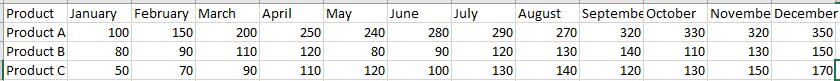
\includegraphics{GraphPic1.png}

\hypertarget{selecting-data-for-the-graph}{%
\subsection{Selecting Data for the Graph}\label{selecting-data-for-the-graph}}

To create a graph, first, select the data you want to include in the chart. In our example, select the cells containing the months and the corresponding sales data for Product A. The data should form a logical range, such as a row or a column.

\hypertarget{inserting-the-graph}{%
\subsection{Inserting the Graph}\label{inserting-the-graph}}

Once the data is selected, follow these steps to insert the graph:

\begin{itemize}
\tightlist
\item
  Click on the ``Insert'' tab in the Excel ribbon at the top of the screen.
\item
  In the Charts group, choose the ``Line Chart'' option (you can select other chart types if you prefer).
\item
  From the drop-down menu, select the specific line chart style you want to use. For this example, choose a basic line chart.
\end{itemize}

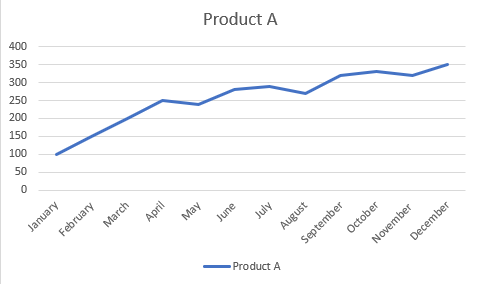
\includegraphics{GraphPic2.png}

\hypertarget{customizing-the-graph}{%
\subsection{Customizing the Graph}\label{customizing-the-graph}}

After inserting the chart, Excel will display it in the worksheet. Now, it's time to customize the graph to make it more informative and visually appealing. Here are some ways to do that:

\begin{itemize}
\item
  Chart Title: Click on the chart title (usually labeled ``Chart Title'') and enter a descriptive title, such as ``Product A Sales over Time.''
\item
  Axis Labels: Click on the horizontal (x-axis) and vertical (y-axis) labels to edit and provide clear descriptions of the data displayed.
\item
  Legend: If Excel didn't automatically add a legend, you can include one by clicking on ``Legend'' in the Chart Elements menu.
\item
  Data Labels: To display the actual data points on the graph, click on ``Data Labels'' in the Chart Elements menu.
\item
  Formatting: Customize the chart's appearance, such as colors, fonts, line styles, and background, to match your preferences or corporate branding.
\end{itemize}

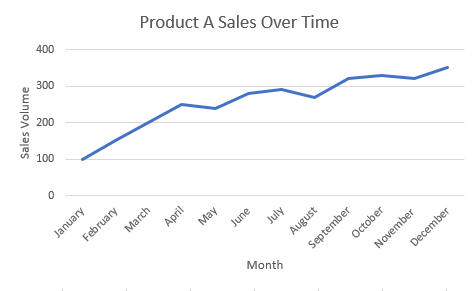
\includegraphics{GraphPic4.png}

\hypertarget{interpreting-the-graph}{%
\subsection{Interpreting the Graph}\label{interpreting-the-graph}}

Once you have customized the graph, take a moment to interpret the insights it provides. In our example, the line chart for Product A sales over time shows whether sales have increased or decreased each month. The line's trend indicates the overall sales trend for Product A, and individual data points show the sales figures for specific months.

\hypertarget{updating-the-graph-with-new-data}{%
\subsection{Updating the Graph with New Data}\label{updating-the-graph-with-new-data}}

One of the advantages of using Excel graphs is their flexibility in handling updated data. If your dataset changes, simply adjust the data range by dragging the handles of the chart or by clicking on ``Select Data'' in the Chart Elements menu. Excel will automatically update the graph with the new data, saving you time and effort.

\hypertarget{conclusion}{%
\section{Conclusion}\label{conclusion}}

Congratulations! You have successfully taken your first steps into the world of Excel graphs. In this chapter, we introduced Microsoft Excel and its graphing capabilities, explored data setup and formatting, and created a simple line chart from scratch. Excel's graphing tools provide a powerful way to visually communicate data insights, making complex information accessible and easy to understand. As you progress through this book, you will explore more chart types, advanced graphing techniques, and best practices to create visually compelling and impactful graphs. Let's continue our journey to Excel Graphs Mastery!

\hypertarget{chart-types-and-when-to-use-them}{%
\chapter{Chart Types and When to Use Them}\label{chart-types-and-when-to-use-them}}

Data visualization is a powerful tool for presenting information effectively and gaining insights from data. Excel offers a wide range of chart types, each designed to highlight different aspects of the data. In this chapter, we will introduce various Excel graphs, explain their purposes, and explore the best use cases for each chart type. We will also provide visual examples with real-world data to demonstrate their applications.

\hypertarget{line-charts}{%
\section{Line Charts}\label{line-charts}}

Purpose: Line charts are used to show trends over time or continuous data series. They are particularly effective for displaying data with a clear sequence, such as sales figures over months or years.

Best Use Cases:

\begin{itemize}
\tightlist
\item
  Visualizing time-series data, such as stock prices, temperature trends, or website traffic over time.
\item
  Comparing multiple data series with a common x-axis, such as sales performance of different products over a period.
\item
  Analyzing trends and identifying patterns in continuous datasets.
\end{itemize}

\hypertarget{bar-charts}{%
\section{Bar Charts}\label{bar-charts}}

Purpose: Bar charts are ideal for comparing discrete categories or data points. They use rectangular bars to represent the values, making it easy to visualize and compare different categories.

Best Use Cases:

\begin{itemize}
\tightlist
\item
  Comparing data between different groups or categories, such as sales performance by different regions or departments.
\item
  Displaying data that does not have a natural order or time component.
\item
  Presenting data with a large number of categories, as bar charts allow for clear differentiation.
\end{itemize}

\hypertarget{pie-charts}{%
\section{Pie Charts}\label{pie-charts}}

Purpose: Pie charts are useful for showing proportions or percentages of a whole. They divide a circle into slices, with each slice representing a different category's proportion of the total.

Best Use Cases:

\begin{itemize}
\tightlist
\item
  Displaying parts of a whole, such as the percentage of sales contributed by different products or the composition of a budget.
\item
  Visualizing categorical data where the relative sizes of the categories are significant.
\end{itemize}

\hypertarget{scatter-plots}{%
\section{Scatter Plots}\label{scatter-plots}}

Purpose: Scatter plots are used to explore relationships and correlations between two numeric variables. Each data point is plotted on the chart, allowing the observation of patterns and trends.

Best Use Cases:

\begin{itemize}
\tightlist
\item
  Identifying relationships between two variables, such as examining the correlation between temperature and ice cream sales.
\item
  Visualizing data points that are not part of a continuous sequence or time-series.
\end{itemize}

\hypertarget{area-charts}{%
\section{Area Charts}\label{area-charts}}

Purpose: Area charts are similar to line charts but emphasize the cumulative total of data over time or a continuous sequence.

Best Use Cases:

\begin{itemize}
\tightlist
\item
  Visualizing trends and variations over time with an emphasis on the total magnitude.
\item
  Comparing the cumulative values of multiple data series.
\end{itemize}

\hypertarget{bar-column-charts}{%
\section{Bar Column Charts}\label{bar-column-charts}}

Purpose: Bar column charts combine the features of bar charts and column charts to visualize data with both positive and negative values.

Best Use Cases:

\begin{itemize}
\tightlist
\item
  Comparing positive and negative values within the same category, such as profit and loss figures for different products.
\item
  Displaying data with both absolute and relative values.
\end{itemize}

\hypertarget{radar-charts}{%
\section{Radar Charts}\label{radar-charts}}

Purpose: Radar charts, also known as spider charts or web charts, are useful for comparing multiple variables across different categories. The chart uses a circular spider-web-like format to display the data.

Best Use Cases:

\begin{itemize}
\tightlist
\item
  Comparing the performance of different entities across various attributes, such as comparing students' scores * across different subjects.
\item
  Visualizing multivariate data and identifying patterns.
\end{itemize}

\hypertarget{bubble-charts}{%
\section{Bubble Charts}\label{bubble-charts}}

Purpose: Bubble charts are an extension of scatter plots, where each data point is represented by a bubble with varying size and color to convey additional information.

Best Use Cases:

\begin{itemize}
\tightlist
\item
  Visualizing three variables in a single chart, where the x-axis and y-axis represent two variables, and the bubble size or color represents the third variable.
\item
  Displaying data points with varying sizes or weights.
\end{itemize}

\hypertarget{conclusion-1}{%
\section{Conclusion}\label{conclusion-1}}

Excel offers a diverse range of chart types, each designed to serve specific purposes and communicate data insights effectively. By understanding the strengths and applications of each chart type, you can choose the most suitable representation for your data and enhance your data visualization skills. As we move forward in this book, you will gain hands-on experience with these chart types, learn advanced graphing techniques, and develop a deeper understanding of data visualization best practices. Let's continue our journey to becoming Excel graphing experts!

\hypertarget{customizing-graphs}{%
\chapter{Customizing Graphs}\label{customizing-graphs}}

Excel graphs are powerful tools for data visualization, but their impact can be enhanced significantly through customization. In this chapter, we will explore how to tailor your Excel graphs to make them visually appealing, informative, and suitable for your specific data. We will cover a range of customization techniques, including modifying chart elements, formatting options, and adjusting scales and axes.

\hypertarget{modifying-chart-elements}{%
\section{Modifying Chart Elements}\label{modifying-chart-elements}}

Customizing chart elements allows you to add context and clarity to your graphs. By labeling and providing essential information, you can help your audience better understand the data. Let's explore how to modify chart elements like titles, axis labels, legends, and data labels:

\hypertarget{chart-titles}{%
\subsection{Chart Titles}\label{chart-titles}}

Adding a descriptive chart title helps viewers understand the graph's purpose at a glance. To modify the chart title:

\begin{itemize}
\tightlist
\item
  Click on the chart to select it.
\item
  Locate and click on the ``Chart Elements'' button (a plus sign or gear icon) that appears when you hover over the chart.
\item
  Check the ``Chart Title'' box to enable the title.
\item
  Click on the newly added title and enter the desired text.
\end{itemize}

\hypertarget{axis-labels}{%
\subsection{Axis Labels}\label{axis-labels}}

Axis labels provide context for the data displayed on the graph. To modify axis labels:

\begin{itemize}
\tightlist
\item
  Click on the chart to select it.
\item
  Locate and click on the ``Chart Elements'' button.
\item
  Check the ``Axis Titles'' box to enable the axis labels for the horizontal (x-axis) and vertical (y-axis) axes.
\item
  Click on each axis label to edit and provide descriptive labels.
\end{itemize}

\hypertarget{legends}{%
\subsection{Legends}\label{legends}}

Legends are especially useful when multiple data series are presented on the same graph. To modify legends:

\begin{itemize}
\tightlist
\item
  Click on the chart to select it.
\item
  Locate and click on the ``Chart Elements'' button.
\item
  Check the ``Legend'' box to enable the legend display.
\item
  Click on the legend to edit and customize its appearance.
\end{itemize}

\hypertarget{data-labels}{%
\subsection{Data Labels}\label{data-labels}}

Data labels display specific data points directly on the chart, making it easier for viewers to interpret the data. To add data labels:

Click on the chart to select it.
* Locate and click on the ``Chart Elements'' button.
* Check the ``Data Labels'' box to enable data labels.
* Customize the data label appearance, such as position, font size, and number formatting.

\hypertarget{formatting-options}{%
\section{Formatting Options}\label{formatting-options}}

Formatting is a crucial aspect of customizing Excel graphs. It allows you to personalize the visual appearance of the chart to match your preferences or your organization's branding. Let's explore some formatting options, such as colors, fonts, and styles:

\hypertarget{colors}{%
\subsection{Colors}\label{colors}}

Colors play a significant role in drawing attention and conveying information. Excel allows you to customize the colors of various chart elements:

\begin{itemize}
\tightlist
\item
  Click on the chart to select it.
\item
  Use the ``Format'' tab that appears in the Excel ribbon when the chart is selected.
\item
  Choose ``Shape Fill'' to modify the background color of chart elements.
\item
  Select ``Shape Outline'' to change the border color of elements.
\item
  Use the ``Font Color'' option to modify the color of text elements like titles and labels.
\end{itemize}

\hypertarget{fonts}{%
\subsection{Fonts}\label{fonts}}

Font selection impacts the readability and overall aesthetic of the chart. To change fonts:

\begin{itemize}
\tightlist
\item
  Click on the chart to select it.
\item
  Use the ``Format'' tab.
\item
  Select the text element you wish to modify, such as titles, axis labels, or data labels.
\item
  Choose a different font and adjust the font size as needed.
\end{itemize}

\hypertarget{styles}{%
\subsection{Styles}\label{styles}}

Excel provides pre-defined chart styles that apply a combination of colors, fonts, and effects to the chart. To apply a chart style:

\begin{itemize}
\tightlist
\item
  Click on the chart to select it.
\item
  Use the ``Chart Styles'' button that appears on the right side of the chart when selected.
\item
  Choose a style from the available options to update the chart's appearance.
\end{itemize}

\hypertarget{adjusting-scales-and-axes}{%
\section{Adjusting Scales and Axes}\label{adjusting-scales-and-axes}}

Adjusting scales and axes is essential to improve the representation of data on the graph. By customizing axis scales, you can ensure that your data is presented in the most suitable and informative manner:

\hypertarget{scaling-options}{%
\subsection{Scaling Options}\label{scaling-options}}

Excel automatically scales the axes based on the data range by default. However, you may sometimes need to set specific scales for better comparison:

\begin{itemize}
\tightlist
\item
  Click on the chart to select it.
\item
  Right-click on the axis you want to modify (x-axis or y-axis).
\item
  Choose ``Format Axis'' from the context menu.
\item
  In the ``Format Axis'' pane, you can customize various options, such as the minimum and maximum values, interval between tick marks, and logarithmic scales.
\end{itemize}

\hypertarget{logarithmic-scale}{%
\subsection{Logarithmic Scale}\label{logarithmic-scale}}

A logarithmic scale is beneficial when dealing with data that covers a wide range of values. It compresses data with large differences, making patterns and trends more apparent:

\begin{itemize}
\tightlist
\item
  Follow the same steps as adjusting the axis scale but select the ``Logarithmic Scale'' option if applicable.
\end{itemize}

\hypertarget{axis-crosses-and-position}{%
\subsection{Axis Crosses and Position}\label{axis-crosses-and-position}}

You can modify the position where the axes intersect and control the axis position to enhance the clarity of the graph:

\begin{itemize}
\tightlist
\item
  Click on the chart to select it.
\item
  Right-click on the axis you want to modify.
\item
  Choose ``Format Axis'' and navigate to the ``Axis Options'' section.
\item
  Adjust the ``Axis Labels'' dropdown to position the axis at the desired location.
\end{itemize}

\hypertarget{secondary-axes}{%
\subsection{Secondary Axes}\label{secondary-axes}}

In some cases, you might need to compare data with different scales on the same chart. Excel allows you to add secondary axes to accommodate this:

\begin{itemize}
\tightlist
\item
  Click on the chart to select it.
\item
  Right-click on one of the data series you want to display on the secondary axis.
\item
  Choose ``Change Series Chart Type'' from the context menu.
\item
  Select the appropriate chart type that supports secondary axes (e.g., line chart) and click ``OK.''
\item
  Right-click on the newly created series and choose ``Format Data Series.''
\item
  In the ``Format Data Series'' pane, choose ``Secondary Axis'' under the ``Plot Series On'' option.
\end{itemize}

\hypertarget{finalizing-your-customization}{%
\section{Finalizing Your Customization}\label{finalizing-your-customization}}

As you customize your Excel graph, remember that balance and simplicity are key to effective data visualization. Avoid overcrowding the chart with unnecessary elements and aim to present data in the most straightforward and meaningful way possible. Always consider your audience and the specific insights you want to communicate.

\hypertarget{conclusion-2}{%
\section{Conclusion}\label{conclusion-2}}

Customizing Excel graphs allows you to transform simple charts into powerful visual representations of data. By modifying chart elements, formatting options, and adjusting scales and axes, you can elevate the visual appeal, clarity, and impact of your graphs significantly. As you progress in your data visualization journey, continue experimenting with customization techniques to create compelling and insightful Excel graphs that effectively communicate your data-driven insights.

\hypertarget{data-analysis-with-excel-graphs}{%
\chapter{Data Analysis with Excel Graphs}\label{data-analysis-with-excel-graphs}}

Excel graphs not only help present data visually but also serve as powerful tools for data analysis. In this chapter, we will explore advanced data analysis techniques using Excel graphs. We will demonstrate how to create combination charts to display multiple data series together, leverage trendlines and error bars to analyze data trends and uncertainties, and add annotations and callouts to highlight essential data points.

\hypertarget{combination-charts-and-secondary-axes}{%
\section{Combination Charts and Secondary Axes}\label{combination-charts-and-secondary-axes}}

Combination charts are valuable when you want to display multiple data series with different scales or data types on the same graph. Additionally, secondary axes can be used to compare data series with distinct units. Let's walk through the process of creating combination charts with secondary axes:

\hypertarget{creating-a-combination-chart}{%
\subsection{Creating a Combination Chart}\label{creating-a-combination-chart}}

To create a combination chart in Excel:

\begin{itemize}
\tightlist
\item
  Select the data you want to include in the chart, including multiple data series with distinct units or scales.
\item
  Click on the ``Insert'' tab in the Excel ribbon.
\item
  Choose the chart type that best suits your data for the first data series (e.g., a column chart).
\item
  Once the chart is inserted, right-click on one of the data series on the chart and select ``Change Series Chart Type.''
\item
  Choose the appropriate chart type for the second data series (e.g., a line chart) from the menu.
\item
  The combination chart will display both data series on the same graph.
\end{itemize}

\hypertarget{adding-a-secondary-axis}{%
\subsection{Adding a Secondary Axis}\label{adding-a-secondary-axis}}

To add a secondary axis to a data series on a combination chart:

\begin{itemize}
\tightlist
\item
  Select the data series you want to display on the secondary axis.
\item
  Right-click on the selected data series and choose ``Format Data Series.''
\item
  In the ``Format Data Series'' pane, select ``Secondary Axis'' under the ``Plot Series On'' option.
\item
  The secondary axis will now appear on the chart, allowing you to compare data series with different scales effectively.
\end{itemize}

\hypertarget{trendlines-and-error-bars}{%
\section{Trendlines and Error Bars}\label{trendlines-and-error-bars}}

Trendlines and error bars are essential tools for analyzing data trends and uncertainties, respectively. Let's explore how to add trendlines and error bars to Excel graphs.

\hypertarget{adding-trendlines}{%
\subsection{Adding Trendlines}\label{adding-trendlines}}

To add a trendline to a data series in Excel:

\begin{itemize}
\tightlist
\item
  Click on the chart to select it.
\item
  Right-click on the data series to which you want to add the trendline.
\item
  Choose ``Add Trendline'' from the context menu.
\item
  The ``Format Trendline'' pane will appear, offering various trendline options.
\item
  Select the desired trendline type, such as linear, exponential, or moving average.
\item
  Customize the trendline appearance and options as needed.
\end{itemize}

\hypertarget{adding-error-bars}{%
\subsection{Adding Error Bars}\label{adding-error-bars}}

To add error bars to a data series in Excel:

\begin{itemize}
\tightlist
\item
  Click on the chart to select it.
\item
  Right-click on the data series to which you want to add error bars.
\item
  Choose ``Add Error Bars'' from the context menu.
\item
  The ``Format Error Bars'' pane will appear, offering options for customizing error bars.
\item
  Select the type of error bars you want to display, such as standard deviation or standard error.
\item
  Customize the error bars' appearance and options, such as line style, cap style, and value range.
\end{itemize}

\hypertarget{annotations-and-callouts}{%
\section{Annotations and Callouts}\label{annotations-and-callouts}}

Annotations and callouts are valuable for highlighting specific data points or providing additional context to the graph. Here's how to add annotations and callouts to Excel graphs.

\hypertarget{adding-annotations}{%
\subsection{Adding Annotations}\label{adding-annotations}}

To add annotations to a data point in Excel:

\begin{itemize}
\tightlist
\item
  Click on the chart to select it.
\item
  Locate and click on the ``Chart Elements'' button (a plus sign or gear icon) that appears when you hover over the chart.
\item
  Check the ``Data Labels'' box to enable data labels on the chart.
\item
  Excel will display data labels on the data points. Click on a data label to edit its text and format.
\item
  You can use annotations to label important data points or provide additional information related to specific data series.
\end{itemize}

\hypertarget{adding-callout}{%
\subsection{Adding Callout}\label{adding-callout}}

To add callouts to a data point in Excel:

\begin{itemize}
\tightlist
\item
  Click on the chart to select it.
\item
  Go to the ``Insert'' tab in the Excel ribbon.
\item
  Choose ``Shapes'' and select the desired callout shape from the dropdown menu.
\item
  Click and drag to draw the callout shape on the chart.
\item
  Enter the text for the callout, which may include explanations or context related to the data.
\item
  Callouts help draw attention to specific data points or provide explanatory notes directly on the graph.
\end{itemize}

\hypertarget{using-data-analysis-tools}{%
\section{Using Data Analysis Tools}\label{using-data-analysis-tools}}

Excel provides additional data analysis tools, such as data tables, pivot charts, and regression analysis, that can further enhance your data analysis capabilities. Here's a brief overview of some of these tools:

\hypertarget{data-tables}{%
\subsection{Data Tables}\label{data-tables}}

Data tables allow you to perform sensitivity analysis by varying input values and observing their impact on the charted data. By creating data tables, you can assess different scenarios and identify critical data points.

\hypertarget{pivot-charts}{%
\subsection{Pivot Charts}\label{pivot-charts}}

Pivot charts enable dynamic data analysis by summarizing and organizing large datasets. By creating pivot charts, you can quickly gain insights and visualize trends in complex data.

\hypertarget{regression-analysis}{%
\subsection{Regression Analysis}\label{regression-analysis}}

Regression analysis helps you determine the relationship between variables and predict future outcomes. By performing regression analysis on your data, you can identify correlations and forecast trends.

\hypertarget{conclusion-3}{%
\section{Conclusion}\label{conclusion-3}}

Excel graphs offer a multitude of data analysis possibilities, enabling users to gain insights and draw meaningful conclusions from their datasets. By creating combination charts with secondary axes, adding trendlines and error bars, and using annotations and callouts, you can elevate the clarity and impact of your data visualizations. Moreover, by employing various data analysis tools provided by Excel, you can delve even deeper into your data to make informed decisions and unlock hidden insights. As you master these techniques, you will become proficient in presenting data with precision and clarity, empowering you to communicate your findings effectively to diverse audiences.

\hypertarget{advanced-graphing-techniques}{%
\chapter{Advanced Graphing Techniques}\label{advanced-graphing-techniques}}

Excel offers a plethora of advanced graphing techniques that take data visualization to new heights. In this chapter, we will explore the more sophisticated features of Excel graphs, including 3D charts, sparklines, and histograms. We will then delve into creating dynamic charts using data tables and named ranges, as well as utilizing pivot charts and slicers for interactive data visualization.

\hypertarget{d-charts-adding-a-new-dimension-to-data-visualization}{%
\section{3D Charts: Adding a New Dimension to Data Visualization}\label{d-charts-adding-a-new-dimension-to-data-visualization}}

3D charts introduce a third dimension to data visualization, providing a unique perspective on data relationships. By adding depth to the chart, 3D charts can reveal patterns and trends that might be less apparent in traditional 2D charts. Excel offers various types of 3D charts, such as 3D column charts, 3D line charts, and 3D surface charts.

To create a 3D chart in Excel:

\begin{itemize}
\tightlist
\item
  Select the data you want to include in the chart.
\item
  Click on the ``Insert'' tab in the Excel ribbon.
\item
  Choose the desired 3D chart type from the ``Charts'' group.
\item
  Excel will insert the 3D chart into your worksheet.
\item
  Customize the chart's appearance and data series as needed.
\end{itemize}

While 3D charts can be visually engaging, exercise caution when using them. In some cases, the additional dimension may distort the data or make it more challenging to interpret accurately. Use 3D charts judiciously, keeping the focus on clarity and data integrity.

\hypertarget{sparklines-tiny-charts-with-big-insights}{%
\section{Sparklines: Tiny Charts with Big Insights}\label{sparklines-tiny-charts-with-big-insights}}

Sparklines are miniature charts that fit within a single cell, providing a quick visual representation of data trends. Sparklines are particularly useful when you want to show data variations or patterns alongside the data itself. Excel supports three types of sparklines: line sparklines, column sparklines, and win/loss sparklines.

To create sparklines in Excel:

\begin{itemize}
\tightlist
\item
  Select the range of data where you want to insert the sparklines.
\item
  Go to the ``Insert'' tab in the Excel ribbon.
\item
  Choose the type of sparkline you want to create from the ``Sparklines'' group.
\item
  Excel will insert the sparklines into each selected cell, visually representing the data trends.
\end{itemize}

Sparklines are an excellent choice for adding compact data visualizations to tables and dashboards, providing immediate insights without taking up much space.

\hypertarget{histograms-unraveling-data-distributions}{%
\section{Histograms: Unraveling Data Distributions}\label{histograms-unraveling-data-distributions}}

Histograms are essential tools for understanding data distributions and frequency. They group data into intervals, called bins, and display the frequency of data points falling within each bin. Histograms are particularly useful when dealing with large datasets and analyzing data patterns.

To create a histogram in Excel:

\begin{itemize}
\tightlist
\item
  Organize the data into a single column in a worksheet.
\item
  Click on the ``Data'' tab in the Excel ribbon.
\item
  Choose ``Data Analysis'' from the ``Data Tools'' group.
\item
  Select ``Histogram'' from the list of data analysis tools and click ``OK.''
\item
  Enter the input range for the data and specify the bin range or let Excel determine the bins automatically.
\item
  Choose the location for the histogram output (new worksheet or existing worksheet) and click ``OK.''
\end{itemize}

Excel will generate a histogram chart that displays the data distribution and allows you to assess data patterns and frequencies.

\hypertarget{dynamic-charts}{%
\section{Dynamic Charts}\label{dynamic-charts}}

Dynamic charts in Excel take data visualization to the next level, providing users with the ability to interactively explore and analyze data. Unlike static charts, dynamic charts update automatically when the underlying data changes, allowing for real-time insights and scenario analysis. In this guide, we will delve into the world of dynamic charts in Excel, exploring how to create them using data tables and named ranges, and understanding their applications and benefits.

\hypertarget{introducing-dynamic-charts}{%
\subsection{Introducing Dynamic Charts}\label{introducing-dynamic-charts}}

Dynamic charts are charts that adapt and change as the underlying data changes. They offer a more interactive and engaging way to visualize data, allowing users to interact with the chart and observe the impact of changing variables on the graph.

\hypertarget{the-power-of-data-tables-for-dynamic-charts}{%
\subsection{The Power of Data Tables for Dynamic Charts}\label{the-power-of-data-tables-for-dynamic-charts}}

Data tables are essential for creating dynamic charts in Excel. A data table is a range of cells that shows how changing one or two variables affects the results of a formula. By using data tables, you can create scenarios and observe the effects of different input values on the charted data.

\hypertarget{creating-data-tables}{%
\subsection{Creating Data Tables}\label{creating-data-tables}}

To create a data table in Excel:

\begin{itemize}
\tightlist
\item
  Set up your data and formulas in a separate worksheet.
\item
  Identify the cell containing the formula that you want to vary.
\item
  Click on the ``Data'' tab in the Excel ribbon.
\item
  Select ``What-If Analysis'' from the ``Data Tools'' group.
\item
  Choose ``Data Table'' from the drop-down menu.
\item
  Enter the cell reference of the cell containing the input value you want to change (e.g., a cell representing growth rate).
\end{itemize}

Excel will automatically populate the data table with different scenarios based on the specified input value.
The chart linked to the data table will update in real-time as you change the input value.

\hypertarget{benefits-of-using-data-tables-for-dynamic-charts}{%
\subsection{Benefits of Using Data Tables for Dynamic Charts}\label{benefits-of-using-data-tables-for-dynamic-charts}}

Using data tables for dynamic charts offers several advantages:

\begin{itemize}
\tightlist
\item
  Real-time Visualization: Data tables provide instant feedback, allowing users to visualize the impact of changes on the charted data immediately.
\item
  Efficient Scenario Analysis: With data tables, users can create multiple scenarios by changing a single input value, enabling easy comparison and analysis of different data variations.
\item
  Interactive Exploration: Dynamic charts with data tables enable users to interact with the data and gain deeper insights by adjusting key parameters.
\end{itemize}

\hypertarget{data-visualization-best-practices}{%
\chapter{Data Visualization Best Practices}\label{data-visualization-best-practices}}

Data visualization is an art that blends science, design, and storytelling to communicate complex information effectively. Excel, as a powerful data analysis tool, provides a wide array of chart types and customization options to create impactful visualizations. In this chapter, we will explore data visualization best practices in Excel, focusing on guidelines for selecting the right chart type for specific data scenarios, color choices, accessibility considerations, and the significance of simplicity, clarity, and accuracy in graph design. By following these best practices, you can transform your Excel charts into compelling and informative visual stories.

\hypertarget{choosing-the-right-chart-type-for-specific-data-scenarios}{%
\section{Choosing the Right Chart Type for Specific Data Scenarios}\label{choosing-the-right-chart-type-for-specific-data-scenarios}}

Selecting the appropriate chart type is the foundation of effective data visualization. Excel offers various chart types, each suited for different data scenarios and communication objectives. Consider the following guidelines when choosing the right chart type:

\hypertarget{understand-the-data}{%
\subsection{Understand the Data}\label{understand-the-data}}

Before selecting a chart type, thoroughly understand your dataset and the insights you want to convey. Identify the variables, their relationships, and any patterns or trends present in the data.

\hypertarget{types-of-chart-types}{%
\subsection{Types of Chart Types}\label{types-of-chart-types}}

Excel provides several chart types, including:

\begin{itemize}
\tightlist
\item
  Column Charts: Suitable for comparing categories and showing changes over time.
\item
  Bar Charts: Ideal for comparing data across different categories.
\item
  Line Charts: Useful for displaying trends and continuous data over time.
\item
  Pie Charts: Appropriate for showing proportions and parts of a whole.
\item
  Scatter Plots: Effective for analyzing relationships between two variables.
\item
  Area Charts: Similar to line charts but visually emphasize the area under the lines.
\item
  Bubble Charts: Combine data points as bubbles to display three variables.
\item
  Radar Charts: Show multivariate data points on a circular grid.
\end{itemize}

\hypertarget{chart-selection-guidelines}{%
\subsection{Chart Selection Guidelines}\label{chart-selection-guidelines}}

Avoid 3D Charts: 3D charts may look visually appealing, but they can distort data and make it challenging to interpret accurately. Stick to 2D charts for clarity.

Keep It Simple: Use simple and familiar chart types to ensure the audience can easily interpret the information.

Highlight Key Insights: Select charts that highlight the most critical insights from your data.

Avoid Overplotting: Avoid cluttering the chart with too many data points, as it may hinder readability.

Utilize Combination Charts: Combine multiple chart types when presenting complex data relationships.

\hypertarget{color-choices-and-accessibility-considerations}{%
\section{Color Choices and Accessibility Considerations}\label{color-choices-and-accessibility-considerations}}

Colors play a vital role in data visualization, influencing perception and highlighting key information. However, it is essential to use colors thoughtfully and consider accessibility for all users. Follow these guidelines for color choices.

\hypertarget{use-a-cohesive-color-palette}{%
\subsection{Use a Cohesive Color Palette}\label{use-a-cohesive-color-palette}}

Limit the number of colors used in a chart to avoid overwhelming the audience.
Choose a cohesive color palette that complements your data and enhances visual appeal.

\hypertarget{emphasize-data-with-color}{%
\subsection{Emphasize Data with Color}\label{emphasize-data-with-color}}

Use color to highlight key data points or categories to draw attention.
Utilize color gradients or heatmaps to represent data variations.

\hypertarget{consider-colorblind-friendly-palettes}{%
\subsection{Consider Colorblind-Friendly Palettes}\label{consider-colorblind-friendly-palettes}}

Around 8\% of men and 0.5\% of women worldwide have some form of color vision deficiency. Choose color palettes that are accessible to colorblind users.
Avoid using red and green together, as these are commonly confused by individuals with red-green color blindness.

\hypertarget{check-contrast-and-readability}{%
\subsection{Check Contrast and Readability}\label{check-contrast-and-readability}}

Ensure sufficient contrast between data elements and background colors to enhance readability.
Test your charts in grayscale to verify that they remain distinguishable without color.

\hypertarget{real-world-scenario-population-distribution}{%
\subsection{Real-World Scenario: Population Distribution}\label{real-world-scenario-population-distribution}}

For instance, when visualizing population distribution across regions, use a color palette with gradual intensity to represent population density. Emphasize high-density areas with darker colors and low-density areas with lighter colors. Ensure that the chosen color palette remains distinguishable for all users, including those with color vision deficiencies.

\hypertarget{emphasizing-simplicity-clarity-and-accuracy-in-graph-design}{%
\section{Emphasizing Simplicity, Clarity, and Accuracy in Graph Design}\label{emphasizing-simplicity-clarity-and-accuracy-in-graph-design}}

Simplicity, clarity, and accuracy are fundamental principles in graph design. These principles ensure that the audience can readily understand the information presented and avoid misinterpretation. Follow these best practices.

\hypertarget{embrace-simplicity}{%
\subsection{Embrace Simplicity}\label{embrace-simplicity}}

Eliminate unnecessary chart elements like excessive gridlines or chart borders to reduce visual clutter.
Avoid using too many colors or decorative elements that do not contribute to the data story.

\hypertarget{prioritize-clarity}{%
\subsection{Prioritize Clarity}\label{prioritize-clarity}}

Use clear and descriptive chart titles, axis labels, and data labels to provide context and understanding.
Choose appropriate font sizes and styles for readability.

\hypertarget{ensure-data-accuracy}{%
\subsection{Ensure Data Accuracy}\label{ensure-data-accuracy}}

Double-check data sources and calculations to prevent inaccuracies in the charts.
Verify that axis scales and intervals accurately represent the data range.

\hypertarget{choose-the-right-chart-elements-for-emphasis}{%
\subsection{Choose the Right Chart Elements for Emphasis}\label{choose-the-right-chart-elements-for-emphasis}}

Utilize data labels, callouts, or annotations to highlight key data points or trends.
Employ the appropriate chart elements, such as trendlines or error bars, to enhance data analysis.

\hypertarget{real-world-scenario-sales-growth-trend}{%
\subsection{Real-World Scenario: Sales Growth Trend}\label{real-world-scenario-sales-growth-trend}}

For instance, when presenting a sales growth trend, use a line chart with clear data labels and a descriptive title. Ensure the chart's axis scales accurately represent the time period to avoid any misinterpretation of growth rates.

\hypertarget{conclusion-4}{%
\section{Conclusion}\label{conclusion-4}}

Effective data visualization in Excel requires a thoughtful approach that aligns with the data scenario, accessibility considerations, and the principles of simplicity, clarity, and accuracy. By choosing the right chart type, using colors strategically, and designing graphs with simplicity and clarity in mind, you can create visualizations that captivate your audience and communicate data-driven insights with precision. Remember that data visualization is a dynamic process, and continuous refinement and iteration are key to presenting information in the most impactful and meaningful way.

\hypertarget{conclusion-5}{%
\chapter{Conclusion}\label{conclusion-5}}

Congratulations! You've completed your journey through the comprehensive textbook on Excel graphs. Throughout this book, we have explored the fascinating world of data visualization using Excel, unlocking the power of visual data communication. From the basics of getting started with Excel graphs to advanced techniques and best practices, you now possess a wealth of knowledge and skills to create compelling and informative visualizations.

\hypertarget{the-impact-of-data-visualization}{%
\section{The Impact of Data Visualization}\label{the-impact-of-data-visualization}}

Data visualization is not merely about creating colorful charts; it is a powerful tool for transforming raw data into meaningful insights. Effective data visualization has the potential to revolutionize decision-making processes, support data-driven strategies, and facilitate communication across diverse audiences. In today's data-driven world, the ability to visualize information effectively is a critical skill, and Excel stands as a versatile and accessible platform for this purpose.

Key Takeaways from Each Chapter

Let's reflect on the key takeaways from each chapter, highlighting the fundamental concepts you've learned:

Chapter 1: Introduction

The purpose of data visualization and its importance in conveying information effectively.
Understanding the role of Excel as a powerful tool for creating various types of graphs.
An overview of the essential topics covered in the book.

Chapter 2: Getting Started with Excel Graphs

How to set up data for graphing, including data formatting and organization.
A step-by-step guide to creating a simple graph from scratch.

Chapter 3: Chart Types and When to Use Them

Introducing different types of Excel graphs and their best use cases.
Providing visual examples of each chart type with real-world data.

Chapter 4: Customizing Excel Graphs

Explaining how to modify chart elements like titles, axis labels, legends, and data labels.
Covering formatting options such as colors, fonts, and styles for better data representation.

Chapter 5: Data Analysis with Excel Graphs

Demonstrating how to create combination charts and secondary axes to display multiple data series together.
Exploring the use of trendlines and error bars to analyze data trends and uncertainties.
Discussing how to add annotations and callouts to highlight important data points.

Chapter 6: Advanced Graphing Techniques

Introducing more advanced features like 3D charts, sparklines, and histograms.
Explaining how to create dynamic charts using data tables and named ranges.
Covering advanced techniques like using pivot charts and slicers for interactive data visualization.

Chapter 7: Data Visualization Best Practices in Excel

Offering guidelines for choosing the right chart type for specific data scenarios.
Discussing color choices and accessibility considerations.
Emphasizing the importance of simplicity, clarity, and accuracy in graph design.

Throughout this textbook, we have emphasized the importance of visual storytelling. Effective data visualization goes beyond presenting charts; it weaves a compelling narrative that engages the audience and guides them to the insights hidden within the data. By adopting best practices, choosing the right chart types, and utilizing design principles, you can craft visual stories that resonate with your audience and drive meaningful action.

\hypertarget{excels-versatility-for-data-visualization}{%
\subsection{Excel's Versatility for Data Visualization}\label{excels-versatility-for-data-visualization}}

Excel has proven to be a versatile and accessible tool for data visualization. Its wide range of chart types, customization options, and advanced features make it an indispensable resource for professionals and enthusiasts alike. Whether you are presenting financial data to stakeholders, analyzing trends for marketing strategies, or visualizing scientific research findings, Excel equips you with the tools to tell your data story effectively.

\hypertarget{continuous-learning-and-exploration}{%
\subsection{Continuous Learning and Exploration}\label{continuous-learning-and-exploration}}

As you conclude this textbook, remember that data visualization is an evolving field. Excel, too, continues to evolve with new updates and features. To stay at the forefront of data visualization, make it a habit to explore new Excel functionalities, attend workshops, and engage with the data visualization community. Continue refining your skills, seeking feedback, and iterating on your visualizations to deliver impactful data stories.

\hypertarget{empowering-decision-making-through-data-visualization}{%
\subsection{Empowering Decision-Making through Data Visualization}\label{empowering-decision-making-through-data-visualization}}

Finally, as you embark on your data visualization journey beyond this textbook, remember the ultimate goal of your work: empowering decision-making through data-driven insights. Your visualizations have the power to unlock the potential of data, guiding businesses, organizations, and individuals towards smarter choices and more significant impacts. Embrace the art and science of Excel graphs, and let your visual stories illuminate the world of data for the better.

  \bibliography{book.bib,packages.bib}

\end{document}
